\chapter*{Johdanto}

1600- ja 1700-luvuilla Suomessa ei ollut rikkaita hoveja suurine muusikkokuntineen. Musiikkielämä ei silti rajoittunut kansanmusiikkiin. Myös oppinutta musiikkia harrastettiin kirkkojen, koulujen, kaupunginpuhaltajien ja sotilassoittokuntien piireissä. Suurimmissa kaupungeissa kuten Turussa, Porissa, Vaasassa ja Viipurissa nämä tahot kykenivät yhdistämään voimansa ja esittämään moniäänistä, jopa monikuoroista musiikkia kirkollisissa ja muissa juhlissa.

Vielä tuohon aikaan musiikki oli tärkeä osa luterilaisten maiden koulusivistystä. Itämeren alueella olikin erityinen, melko yhtenevä koulumusiikkiohjelmisto, johon tutustuminen korjaa sitä yleistä virhekäsitystä, että entisaikaan olisi esitetty vain uutta musiikkia. Suosituinta koulumusiikkia eivät suinkaan olleet ajan tunnetuimpien säveltäjien uudenaikaisimmat luomukset, vaan 1500-luvun ja 1600-luvun alun vokaalipolyfonia. Vanhakantaisuus ei ollut osoitus Pohjolan taantumuksellisuudesta, sillä samaa perinteistä ohjelmistoa käytti myös esimerkiksi Bach Leipzigissä.

Tärkein, joskin edelleen huonosti tunnettu todistus Suomessa harjoitetusta koulumusiikista ovat Porin triviaalikoulun nuottikirjat, jotka Heikki Klemetti löysi Porin Lyseon kirjastosta yli sata vuotta sitten. Nämä neljä äänikirjaa on kopioitu käsin vuonna 1725 triviaalikoulun käyttöön, mahdollisesti korvaamaan isovihan aikana hävitettyjä aiempia nuottikirjoja, ja ne sisältävät 4-, 5- ja 8-äänistä hengellistä vokaalimusiikkia. Kokoelman 93 sävellystä ovat latinan- ja ruotsinkielisiä. Vain yksi, Melchior Vulpiuksen Matteus-passio vuodelta 1613, on suomeksi käännetty. Sama teos on säilynyt lukuisissa muissakin suomalaisissa lähteissä ja sillä oli Suomessa yli sata vuotta yhtäjaksoisesti kestänyt esitysperinne.

Vulpiuksen passio on myös ainoa Porin nuottikirjoihin sisältyvä teos, jonka säveltäjä on nimeltä mainittu. Äänikirjojen kopioija ei nähtävästi pitänyt säveltäjätietoja tärkeinä, eikä montaakaan kappaleen säveltäjää ole vielä kyetty nimeämään. Lukuisat venetsialaistyyliset kaksoiskuoromotetit ovat tunnistettavissa slovenialaissyntyisen Jacobus Galluksen teoksiksi. Galluksen musiikkia on runsaasti myös kuuluisassa Florilegium Portense -kokoelmassa, jota myös Bach käytti. Toinen Suomessa suosittu koulusäveltäjä oli Rostockin urkuri Daniel Friderici, jonka sävellyksiä on myös Piae Cantiones -kokoelman vuoden 1625 painoksessa.

Eräät nuottikirjojen sävellykset ovat vanhoja populaarisävelmiä, joihin on sepitetty uusi, hengellinen teksti. Nunc zymphonizate on alun perin Giovanni Gastoldin balletto La sirena. Christus factus est pro nobis taas on alkujaan instrumentaalinen pavana La Bataille, joka puolestaan lainaa Clément Janequinin samannimistä chansonia vuodelta 1515. Susanna se videns kertoo olennaisimman osan Vanhan Testamentin apokryfikirjoihin sisältyvästä Susannan ja vanhimpien tarinasta, joka tunnettiin eri puolilla Eurooppaa Orlando di Lasson viisiäänisenä, runsaan polyfonisena madrigaalina. Porin nuottikirjoihin on kuitenkin valittu Didier Lupin yksinkertainen neliääninen versio. Tämä ratkaisu on luonteenomaista koulumusiikkikokoelmille, joissa tarkoituksella vältettiin monimutkaista polyfoniaa. Silti monet Porin äänikirjoihin sisältyvät sävellykset ovat taitavasti tehtyjä ja musiikillisesti vaikuttavia. Eräät äänenkuljetuksellisesti kömpelöt kappaleet saattavat olla paikallisten muusikoitten työtä jommalta kummalta puolen Pohjanlahtea.

\section*{Modernisoitu editio: Uusi Porin Triviaalikoulun nuottikirja}

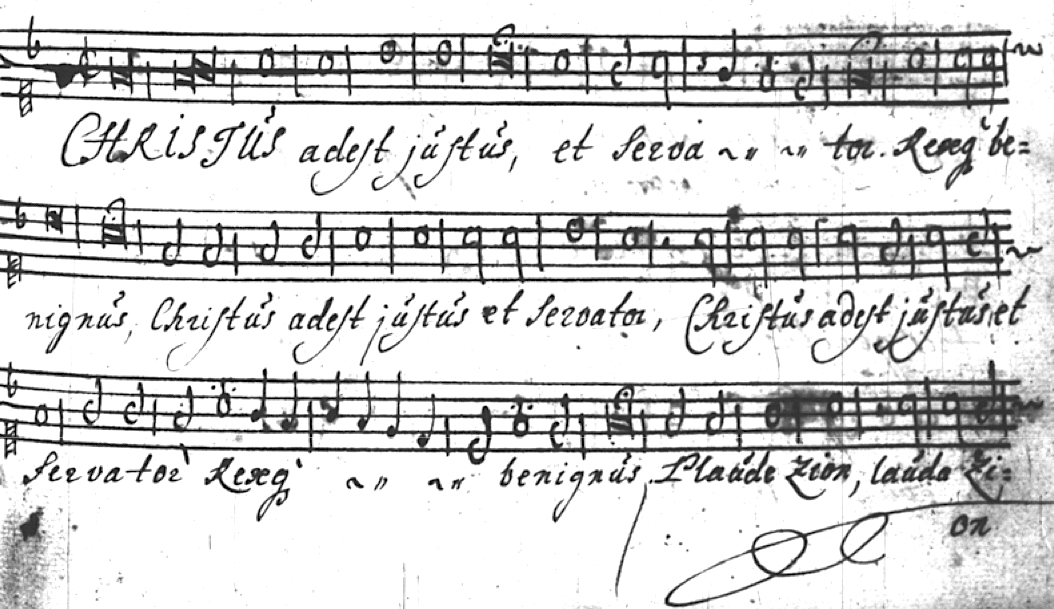
\includegraphics[scale=0.35]{../facsimile/christus-adest-justus}

Nyt julkaistu editio Porin Triviaalikoulun nuottikirjoista vuodelta 1725 on 29 kappaleen valikoima, joita soitin- ja lauluyhtye Sonus Borealis on esittänyt konserteissaan sekä levyjulkaisussaan \textit{Musiikkia Porin Triviaalikoulun nuottikirjoista} (2008). Tämä on ensimmäinen modernisoitu nuottikirjasta tehty kokoelma. Kirja on painettu omakustanteena ja on saatavilla myös verkosta avoimella CC0-lisenssillä osoitteessa \url{https://triviaalikoulu.sonusborealis.fi}. Verkkoversiota päivitetään jatkuvasti ja sieltä voi ladata yksittäisten kappaleiden ja stemmojen nuotit. Teosta voi lupaa pyytämättä kopioida, muokata, levittää ja esittää, mukaan lukien kaupallisessa tarkoituksessa.

Sonus Borealis -yhtyeen perustaja ja taiteellinen johtaja Johannes Vesterinen on rekonstruoinut ja modernisoinut valikoidut kappaleet esityskäyttöä varten käyttäen lähteenään Helsingin yliopiston kirjaston mikrofilminäköispainosta. Tämä julkaisu on siis ymmärryksellä ja asiantuntemuksella tehty käyttöjulkaisu vanhan pohjalta, ei tieteellinen tai kriittinen editio -- eli eräänlainen Uusi Porin Triviaalikoulun nuottikirja nykypäivän käyttöön.

Modernisoinnin yhteydessä kappaleet on kirjoitettu puhtaaksi nykyaikaisella notaatiolla ja niistä on lisäksi korjattu ilmeisimmät musiikilliset virheet, jotka ovat voineet syntyä myös alkuperäisen nuottilähteen käsin tehdyssä puhtaaksikirjoitusvaiheessa. Ainoa selvästi alkuperäislähteestä poikkeava on Vesterisen sovitus neliäänisestä kappaleesta Veni Sancte Spiritus aivan edition lopussa. Se on eräänlainen tarjoiluehdotus 1700-luvun rikkaan sävelkielen tarjoamista variaatioiden runsaudesta ja harmonisesta svengistä.

Rekonstruoinnissa ison osa työstä on muodostanut alkuperäisen, käsin kirjoitettujen latinan- ja ruotsinkielisten laulutekstien tulkitseminen ja tavuttaminen nuotinnokseen sopivaksi. Kolmen kappaleen osalta editioon on lisätty myös toisista lähteistä löytyneet suomenkieliset tekstit: Ainoan Jumalan corkeudes (Allenaste Gud i himmelrik), Äänel caunist monen mutcain (Ætas carmen melodiæ), tuiman talven taucomast (Cedit hyems eminus) sekä Ain iloidca, ain riemuidca (Jugundare jugiter).

Puhtaaksikirjoituksessa suurena apuna on ollut Jyväskylän yliopiston facsimile-julkaisu (2009; Viergutz, Gudrun) sekä lisäksi toissijaiset nuottilähteet Florilegium Portense I ja II (1618 ja 1621; Bodenschatz, Erhard), Psalm-singende Und Lobgesäng-spielende Kirche Christi In Des H. Röm. Reichs (1704, Helmhack, Erasmus), Wanhain Suomen maan pijspain ja Kircon Esimiesten Latinan kielised laulud (1616; Maskulainen, Hemminki), Piae Cantiones (1625, Rutha, Theodoricus Petri sekä Mats Lillhannuksen editio), Then Svenska Psalmboken (1695), Uusi Suomenkielinen Wirsi-Kirja (1701) ja Viridarium music sacrum, sive Cantiones Sacrae, quaternis et quinis vocibus (1625; Daniel Friderici).

Toiveenamme on tällä työllä juhlistaa alkuperäisen nuottikirjan 300. merkkivuotta, nostaa sen sisältämää vanhaa musiikkia esiin ja edistää sen esittämistä ja jalostumista uusiksi tulkinnoiksi. Soiton ja laulun iloa!

\textit{Teksti: Jaakko Saarinen ja Yrjö Kari-Koskinen}
